\section[Ausfall]{Ausgefallenes Material}

\begin{frame}
  {Flexion und Klausur}
  \pause
  \begin{itemize}[<+->]
    \item Der letztes Mal wegen der technischen Probleme\\
      ausgefallene Stoff kann nicht live nachgeholt werden.
    \item \alert{Kapitel 9 und 10 sind absolut elementar.}
    \item \rot{Kapitel 9 und 10 sind Klausurstoff.}
  \end{itemize}
\end{frame}

% \section{Rückblick}
% 
% \begin{frame}[<+->]
%   {Wortbildung vs.\ Flexion}
%   \pause
%   \begin{itemize}
%     \item Flexion als Mittel zur Dekodierung von Struktur (z.\,B.\ Kasus)
%     \item Flexion als Mittel zur Kodierung semantischer Effekte (z.\,B.\ Numerus)
%     \item Wortbildung als Mittel der Wortschatzerweiterung und -optimierung
%       \Halbzeile
%     \item Markierungsfunktion von Morphen:\\
%       \alert{Einschränkung} der möglichen Funktion
%     \item Stämme: mit lexikalischer Markierungsfunktion
%     \item Affixe: ohne lexikalische Markierungsfunktion; nicht wortfähig
%       \Halbzeile
%     \item Wortbildung (gegenüber Flexion)
%       \begin{itemize}
%         \item Änderung statische Merkmale
%         \item Bildung neuer lexikalischer Wörter
%         \item meist (semantisch und formal) eingeschränkte Anwendbarkeit
%       \end{itemize} 
%   \end{itemize}
% \end{frame}

\section{Überblick}

\begin{frame}
  {Warum über Flexion sprechen?}
  \pause
  \begin{itemize}[<+->]
    \item \alert{Wir beherrschen doch alle Formen!}
      \Halbzeile
    \item Funktion der Flexionskategorien
      \begin{itemize}
        \item semantisch\slash pragmatisch
        \item \alert{systemintern} als Hilfe zu \alert{Rekonstruktion der Satzstruktur}
      \end{itemize}
      \Halbzeile
    \item Flexion im Deutschen ein ideales und gut durchschaubares Beispiel\\
      für die klassische \alert{reduktionistische} Methode der Linguistik\\
      (= Analyse der Sprache als \alert{System})
      \Halbzeile
    \item \alert{Können} vs.\ \rot{Erklären}
    \item Reaktion auf Erwerbsschwierigkeiten (L1)
    \item inkl.\ Schwierigkeiten wegen nicht-deutscher Erstsprache (L2)
      \Halbzeile
    \item Heute keine Beispiele? Doch, aber es sind ganze Paradigmen!
%    \item Habe ich eigtl.\ schonmal erzählt, wie ich Kasus verstanden habe?
  \end{itemize}
\end{frame}

% \begin{frame}
%   {Übrigens}
%   \pause
%   \centering
%   \Large
%   \alert{Lesen Sie irgendwann in Ihrem Leben Kapitel 5\\
%     aus Peter Eisenbergs \textit{Grundriss}: \textit{Das Wort}.}\\
%     \Halbzeile
%     (konkret: \citealt[145--200]{Eisenberg2013a})
% \end{frame}

\section{Umlaut und Ablaut}

\begin{frame}
  {Umlaut vs.\ Ablaut: Warum erst jetzt?}
  \pause
  \alert{"`So ein chaotisches Buch! Plötzlich geht es\\
  in der Morphologie wieder um Phonologie!"'}\pause --- Ja\dots
  \pause
  \Zeile
  \begin{itemize}[<+->]
    \item Morphophonologie
    \item Morphosyntax
    \item Syntax-Semantik-Schnittstelle
    \item Prosodie-Pragmatik-Schnittstelle
    \item usw.
      \Zeile
    \item \rot{Die Grammatik nutzt die verfügbaren Mittel gut aus,\\
      und Markierungsmöglichkeiten aller Ebenen können\\
    auf anderen Ebenen zum Einsatz kommen.}
  \end{itemize}
\end{frame}

\begin{frame}[fragile]
  {Umlaut}
  \pause
  \begin{center}
    \resizebox{0.4\textwidth}{!}{
    \begin{tikzpicture}[scale=3.5,baseline=default]
      \large
      \tikzset{
        vowel/.style={fill=white, anchor=mid, text depth=0ex, text height=1ex},
        vowelgespannt/.style={circle,fill=gray!30, anchor=mid, text depth=0ex, text height=1ex,minimum size=4ex},
        dot/.style={circle,fill=black,minimum size=0.4ex,inner sep=0pt,outer sep=-1pt},
      }

      \coordinate (hf) at (0,2); % high front
      \coordinate (hb) at (2,2); % high back
      \coordinate (lf) at (1,0); % low front
      \coordinate (lb) at (2,0); % low back
      \def\V(#1,#2){barycentric cs:hf={(3-#1)*(2-#2)},hb={(3-#1)*#2},lf={#1*(2-#2)},lb={#1*#2}}

      % Chart key (vorne -- hinten).
      \draw [{Latex[round]}-] (\V (-.25,0)) -- (\V (-.25,.5)) node[above left] {\footnotesize vorne};
      \draw [-{Latex[round]}] (\V (-.25,1.5)) -- (\V (-.25,2)) node[above left] {\footnotesize hinten};
      \path (\V (-.25,1)) node[above] {\footnotesize zentral};

      % Chart key (hoch -- tief).
      \draw [{Latex[round]}-] (\V (0,-.25)) -- +(270:.5cm) node[above right,rotate=90] (vokaltrapez1) {\footnotesize hoch};
      \draw [{Latex[round]}-] (\V (3,-2.5)) -- +(270:-.5cm) node[above left,rotate=90] (vokaltrapez2) {\footnotesize tief};
      \path (\V (1.5,-1)) node[above,rotate=90] {\footnotesize mittel};

      % Grid.
      \draw [gray, thick] (\V(0,0)) -- (\V(0,2));
      \draw [gray, thick] (\V(3,0)) -- (\V(3,2));
      \draw [gray, thick] (\V(0,0)) -- (\V(3,0));
      \draw [gray, thick] (\V(0,2)) -- (\V(3,2));

      % Vowels.
      \path (\V (0,2))     node[vowelgespannt] (u)   {u};
      \path (\V(0,0))      node[vowelgespannt] (y)   {y};
      \path (\V (0.5,1.5)) node[vowel]         (uu)  {ʊ};
      \path (\V(0.5,0.5))  node[vowel]         (yy)  {ʏ};
      \path (\V (1,2))     node[vowelgespannt] (o)   {o};
      \path (\V(1.25,0))   node[vowelgespannt] (oe)  {ø};
      \path (\V(3,1))      node[vowelgespannt] (a)   {a};
      \path (\V(2,0))      node[vowelgespannt] (ee)  {ɛ};
      \path (\V(2.5,1))    node[vowel]         (aa)  {ă};
      \path (\V(1.65,0.5)) node[vowel]         (eee) {ɛ̆};
      \path (\V (1.5,1.4)) node[vowel]         (oo)  {ɔ};
      \path (\V(1.4,0.5))  node[vowel]         (oee) {œ};

      \only<3>{\path (u)  edge [-{Latex[round]}, bend left=10]  (y);}
      \only<4>{\path (uu) edge [-{Latex[round]}, bend left=10]  (yy);}
      \only<5>{\path (o)  edge [-{Latex[round]}, bend right=10] (oe);}
      \only<6>{\path (oo) edge [-{Latex[round]}, bend right=5]  (oee);}
      \only<7>{\path (aa) edge [-{Latex[round]}, bend right=10] (eee);}
      \only<8>{\path (a)  edge [-{Latex[round]}, bend left=10]  (ee);}
      
      \only<9->{\path (u)  edge [-{Latex[round]}, bend left=10]  (y);
        \path (uu) edge [-{Latex[round]}, bend left=10]  (yy);
        \path (o)  edge [-{Latex[round]}, bend right=10] (oe);
        \path (oo) edge [-{Latex[round]}, bend right=5]  (oee);
        \path (aa) edge [-{Latex[round]}, bend right=10] (eee);
        \path (a)  edge [-{Latex[round]}, bend left=10]  (ee);}
    \end{tikzpicture}
    }
  \end{center}
  \raggedleft
  \only<3>{G\rot{u}t [g\rot{uː}t] -- G\rot{ü}ter [g\rot{yː}tɐ]\AbUmlautBreaker}
  \only<4>{M\rot{u}tter [m\rot{ʊ}tɐ] -- M\rot{ü}tter [m\rot{ʏ}tɐ]\AbUmlautBreaker}
  \only<5>{T\rot{o}n [t\rot{oː}n]-- T\rot{ö}ne [t\rot{øː}nə]\AbUmlautBreaker}
  \only<6>{\rot{o}ft [ʔ\rot{ɔ}ft] -- \rot{ö}fter [ʔ\rot{œ}ftɐ]\AbUmlautBreaker}
  \only<7>{kr\rot{a}nk [kʁ\rot{a}ŋk] -- kr\rot{ä}nker [kʁ\rot{ɛ}ŋkɐ]\AbUmlautBreaker}
  \only<8>{B\rot{a}d [b\rot{aː}t] -- B\rot{ä}der [b\rot{ɛ}dɐ]}
  \ifdefined\HANDOUT
    \newline
  \fi
  \onslide<9->{Ein vorhersagbarer Prozess: \alert{Frontierung!}}
\end{frame}

\begin{frame}[fragile]
  {Vokalstufen (überwiegend Ablaut)}
  \pause
  Eine kleine Auswahl der möglichen Reihen von Vokalstufen\ldots
  \pause
  \begin{center}
    \resizebox{0.4\textwidth}{!}{
    \begin{tikzpicture}[scale=3.5,baseline=default]
      \large
      \tikzset{
        vowel/.style={fill=white, anchor=mid, text depth=0ex, text height=1ex},
        dot/.style={circle,fill=black,minimum size=0.4ex,inner sep=0pt,outer sep=-1pt},
      }

      \coordinate (hf) at (0,2); % high front
      \coordinate (hb) at (2,2); % high back
      \coordinate (lf) at (1,0); % low front
      \coordinate (lb) at (2,0); % low back
      \def\V(#1,#2){barycentric cs:hf={(3-#1)*(2-#2)},hb={(3-#1)*#2},lf={#1*(2-#2)},lb={#1*#2}}

      % Chart key (vorne -- hinten).
      \draw [{Latex[round]}-] (\V (-.25,0))   -- (\V (-.25,.5)) node [above left] {\footnotesize vorne};
      \draw [-{Latex[round]}] (\V (-.25,1.5)) -- (\V (-.25,2))  node [above left] {\footnotesize hinten};
      \path (\V (-.25,1)) node[above] {\footnotesize zentral};

      % Chart key (hoch--tief).
      \draw [{Latex[round]}-] (\V (0,-.25)) -- +(270:.5cm)  node [above right,rotate=90] (vokaltrapez1) {\footnotesize hoch};
      \draw [{Latex[round]}-] (\V (3,-2.5)) -- +(270:-.5cm) node [above left,rotate=90] (vokaltrapez2) {\footnotesize tief};
      \path (\V (1.5,-1)) node[above,rotate=90] {\footnotesize mittel};

      % Grid. 
      \draw [gray, thick] (\V(0,0)) -- (\V(0,2));
      \draw [gray, thick] (\V(1,0)) -- (\V(1,2));
      \draw [gray, thick] (\V(2,0)) -- (\V(2,2));
      \draw [gray, thick] (\V(3,0)) -- (\V(3,2));
      \draw [gray, thick] (\V(0,0)) -- (\V(3,0));
      \draw [gray, thick] (\V(0,1)) -- (\V(3,1));
      \draw [gray, thick] (\V(0,2)) -- (\V(3,2));

      % Unrounded-rounded pairs.
      \path (\V(0,0))     node [vowel] (i)   {i};
      \path (\V(0.5,0.5)) node [vowel] (I)   {ɪ};   
      \path (\V(1,0))     node [vowel] (e)   {e};
      \path (\V(2,0))     node [vowel] (E)   {ɛ};

      % Unpaired symbols.
      \path (\V(3,1))      node [vowel] (a)  {a};
      \path (\V (2,2))     node [vowel] (oo) {ɔ};
      \path (\V (1,2))     node [vowel] (o)  {o};
      \path (\V (0,2))     node [vowel] (u)  {u};
      \path (\V (0.5,1.5)) node [vowel] (uu) {ʊ};

      \only<4>{\path (i)  edge [red, *-{Latex[round, width=5pt]}, bend left=10] (o);}
      \only<5>{\path (e)  edge [cyan, *-{Latex[round, width=5pt]}, bend left=10] (o);}
      \only<6>{\path (I)  edge [blue, *-, bend right=10] (a);\path (a)  edge [blue, -{Latex[round, width=5pt]}, bend right=10] (uu);}
      \only<7>{\path (E)  edge [green, *-{Latex[round, width=5pt]}, bend right=10] (a);\path (a)  edge [green, -{Latex[round, width=5pt]}, bend right=10] (oo);}
      \only<8>{\path (a)  edge [brown, *-, bend right=10] (u);\path (u)  edge [brown, -{Latex[round, width=5pt]}, bend right=10] (a);}
      \only<9>{\path (I)  edge [orange, *-{Latex[round, width=5pt]}, bend right=10] (uu);}
      \only<10>{\path (I)  edge [purple, *-, bend left=10] (a);\path (a)  edge [purple, -{Latex[round, width=5pt]}, bend right=10] (E);}

      \only<11>{\path (i)  edge [red, *-{Latex[round, width=5pt]}, bend left=10] (o);
        \path (e)  edge [cyan, *-{Latex[round, width=5pt]}, bend left=10] (o);
        \path (I)  edge [blue, *-, bend right=10] (a);\path (a)  edge [blue, -{Latex[round, width=5pt]}, bend right=10] (uu);
        \path (E)  edge [green, *-{Latex[round, width=5pt]}, bend right=10] (a);\path (a)  edge [green, -{Latex[round, width=5pt]}, bend right=10] (oo);
        \path (a)  edge [brown, *-, bend right=10] (u);\path (u)  edge [brown, -{Latex[round, width=5pt]}, bend right=10] (a); 
        \path (I)  edge [purple, *-, bend left=10] (a);\path (a)  edge [purple, -{Latex[round, width=5pt]}, bend right=10] (E);
      \path (I)  edge [orange, *-{Latex[round, width=5pt]}, bend right=10] (uu);}


    \end{tikzpicture}
    }
  \end{center}
  \raggedleft
  \ifdefined\HANDOUT
    \tiny
  \fi
  \only<4>{fr\textcolor{red}{ie}ren [fʁ\textcolor{red}{iː}ʁən] -- fr\textcolor{red}{o}r [fr\textcolor{red}{oː}͡ɐ] -- gefr\textcolor{red}{o}ren [gəfr\textcolor{red}{oː}ʁən]\AbUmlautBreaker}
  \only<5>{h\textcolor{cyan}{e}ben [h\textcolor{cyan}{eː}bən] -- h\textcolor{cyan}{o}b [h\textcolor{cyan}{oː}p] -- geh\textcolor{cyan}{o}ben [gəh\textcolor{cyan}{oː}bən]\AbUmlautBreaker}
  \only<6>{b\textcolor{blue}{i}nden [b\textcolor{blue}{ɪ}ndən] -- b\textcolor{blue}{a}nd [b\textcolor{blue}{a}nt] -- geb\textcolor{blue}{u}nden [gəb\textcolor{blue}{ʊ}ndən]\AbUmlautBreaker}
  \only<7>{b\textcolor{green}{e}rgen [b\textcolor{green}{ɛ}͡əgən] -- b\textcolor{green}{a}rg [b\textcolor{green}{a}͡ək] -- geb\textcolor{green}{o}rgen [gəb\textcolor{green}{ɔ}͡əgən]\AbUmlautBreaker}
  \only<8>{sch\textcolor{brown}{a}ffen [ʃ\textcolor{brown}{a}fən] -- sch\textcolor{brown}{u}f [ʃ\textcolor{brown}{uː}f] -- gesch\textcolor{brown}{a}ffen [gəʃ\textcolor{brown}{a}fən]\AbUmlautBreaker}
  \only<9>{sch\textcolor{orange}{i}nden [ʃ\textcolor{orange}{ɪ}ndən] -- sch\textcolor{orange}{u}nd [ʃ\textcolor{orange}{ʊ}nt] -- gesch\textcolor{orange}{u}nden [gəʃ\textcolor{orange}{ʊ}ndən]\AbUmlautBreaker}
  \only<10>{s\textcolor{purple}{i}tzen [z\textcolor{purple}{ɪ}t͡sən] -- s\textcolor{purple}{a}ß [z\textcolor{purple}{aː}s] -- ges\textcolor{purple}{e}ssen [gəz\textcolor{purple}{ɛ}sən]}
  \ifdefined\HANDOUT
    \newline
  \fi
  \onslide<11->{\rot{Kein vorhersagbarer Prozess!} Lexikalisch\slash verbklassenbasiert.}
\end{frame}


\section{Nominalflexion}

\subsection{Substantive}

\begin{frame}
  {Substantive: Kasus und Numerus}
  Das traditionelle Chaos der Flexionstypen mit Kasus-Numerus-Formen\ldots\\
  \Zeile
  \pause
  \Zeile
  \resizebox{\textwidth}{!}{
    \begin{tabular}{llp{0mm}lp{2mm}llp{1mm}lp{2mm}llp{2mm}l}
      \toprule
      \multicolumn{2}{c}{} && \multicolumn{1}{l}{\textbf{Maskulinum}} && \multicolumn{4}{l}{\textbf{Maskulinum und Neutrum}} && \multicolumn{2}{l}{\textbf{Femininum}} && \multicolumn{1}{l}{\textbf{s-Flexion}} \\
      \multicolumn{2}{c}{} && \multicolumn{1}{l}{\textbf{schwach (S1)}} && \multicolumn{2}{l}{\textbf{stark (S2)}} && \multicolumn{1}{l}{\textbf{gemischt (S3)}} && \multicolumn{2}{l}{\textbf{(S4)}} && \multicolumn{1}{l}{\textbf{(S5)}} \\
      \midrule
      \multirow{4}{*}{\textbf{Sg}} & \textbf{Nom} && Mensch && Stuhl & Haus && Staat && Frau & \multicolumn{1}{l}{Sau} && Auto \\
      & \textbf{Akk} && Mensch-en && Stuhl & Haus && Staat && Frau & \multicolumn{1}{l}{Sau} && Auto \\
      & \textbf{Dat} && Mensch-en && Stuhl & Haus && Staat && Frau & \multicolumn{1}{l}{Sau} && Auto \\
      & \textbf{Gen} && Mensch-en && Stuhl-es & Haus-es && Staat-(e)s && Frau & \multicolumn{1}{l}{Sau} && Auto-s \\
      \midrule
      \multirow{4}{*}{\textbf{Pl}} & \textbf{Nom} && Mensch-en && Stühl-e & Häus-er && Staat-en && Frau-en & \multicolumn{1}{l}{Säu-e} && Auto-s \\
      & \textbf{Akk} && Mensch-en && Stühl-e & Häus-er && Staat-en && Frau-en & \multicolumn{1}{l}{Säu-e} && Auto-s \\
      & \textbf{Dat} && Mensch-en && Stühl-en & Häus-ern && Staat-en && Frau-en & \multicolumn{1}{l}{Säu-en} && Auto-s \\
      & \textbf{Gen} && Mensch-en && Stühl-e & Häus-er && Staat-en && Frau-en & \multicolumn{1}{l}{Säu-e} && Auto-s \\
      \bottomrule
    \end{tabular}
  }
\end{frame}

\begin{frame}
  {Das traditionelle Chaos als "`System"'}
  \pause
  Das geht irgendwie nach Genus und Pluralbildung, aber nicht nur\ldots\\
  \pause
  \Zeile
  \begin{center}
    \resizebox{0.8\textwidth}{!}{
    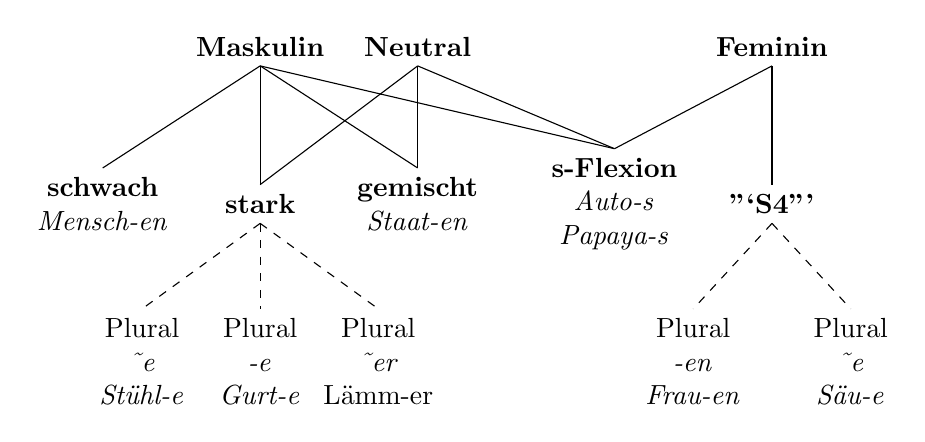
\begin{tikzpicture}[every text node part/.style={align=center}]
      \node (MaskN)    at (2,4)   {\textbf{Maskulin}};
      \node (NeutN)    at (4,4)   {\textbf{Neutral}};
      \node (FemN)     at (8.5,4) {\textbf{Feminin}};

      \node (schwachN) at (0,2)   {\textbf{schwach}\\\textit{Mensch-en}};
      \node (starkN)   at (2,2)   {\textbf{stark}};
      \node (gemistN)  at (4,2)   {\textbf{gemischt}\\\textit{Staat-en}};
      \node (sFlexN)   at (6.5,2) {\textbf{s-Flexion}\\\textit{Auto-s}\\\textit{Papaya-s}};
      \node (s4N)      at (8.5,2) {\textbf{"`S4"'}};

      \node (EPlu)     at (0.5,0) {Plural\\\textit{\char`~e}\\\textit{Stühl-e}};
      \node (ePlu)     at (2,0)   {Plural\\\textit{-e}\\\textit{Gurt-e}};
      \node (erPlu)    at (3.5,0) {Plural\\\textit{\char`~er}\\Lämm-er};

      \node (enPlu)    at (7.5,0) {Plural\\\textit{-en}\\\textit{Frau-en}};
      \node (EnPlu)    at (9.5,0) {Plural\\\textit{\char`~e}\\\textit{Säu-e}};

      \draw (MaskN.south)  -- (schwachN.north);
      \draw (MaskN.south)  -- (starkN.north);
      \draw (MaskN.south)  -- (gemistN.north);
      \draw (MaskN.south)  -- (sFlexN.north);

      \draw (NeutN.south)  -- (starkN.north);
      \draw (NeutN.south)  -- (gemistN.north);
      \draw (NeutN.south)  -- (sFlexN.north);

      \draw (FemN.south)   -- (s4N.north);
      \draw (FemN.south)   -- (sFlexN.north);

      \draw [dashed] (starkN.south) -- (EPlu.north);
      \draw [dashed] (starkN.south) -- (ePlu.north);
      \draw [dashed] (starkN.south) -- (erPlu.north);

      \draw [dashed] (s4N.south)    -- (enPlu.north);
      \draw [dashed] (s4N.south)    -- (EnPlu.north);
    \end{tikzpicture}
  }      
  \end{center}
\end{frame}

\begin{frame}
  {Aber das war noch nicht alles: mit und ohne Schwa}
  \pause
  Es gibt außerdem noch Varianten der Affixe \rot{ohne Schwa}:\\
  \Zeile
  \pause
  \begin{center}
    \resizebox{\textwidth}{!}{
      \begin{tabular}{llp{1mm}llp{1mm}llp{1mm}ll}
        \toprule
        \multicolumn{2}{l}{\textbf{schwach}} && \multicolumn{2}{l}{\textbf{gemischt}} && \multicolumn{2}{l}{\textbf{Fem S4a}} && \multicolumn{2}{l}{\textbf{Fem S4b}}\\
        \textbf{voll} & \textbf{reduziert} && \textbf{voll} & \textbf{reduziert} && \textbf{voll} & \textbf{reduziert} && \textbf{voll} & \textbf{reduziert} \\
        \midrule
        Mensch\alert{-en} & Löwe\rot{-n} && Staat\alert{-en} & Ende\rot{-n} && Frau\alert{-en} & Nudel\rot{-n} && Säu\alert{-e} & Mütter\rot{-$\emptyset$} \\
        \bottomrule
      \end{tabular}
    }
  \end{center}
\end{frame}


% \begin{frame}
%   {Der Ansatz in EGBD}
%   \large \alert{Sauber trennen zwischen Numerus- und Kasusmarkierung!}\\
%   \pause
%   \Halbzeile
%   \normalsize
%   Erstens: Der Plural ist nahezu immer \orongsch{stärker markiert} als\\
%   oder mindestens \gruen{gleich stark markiert} wie der Singular.\\
%   → Pluralbildung ist die \alert{dominante Flexionseigenschaft}.
%   \pause
%   \Zeile
%   \begin{center}
%     \scalebox{0.8}{
%       \begin{tabular}{llll}
%         \toprule
%         \textbf{Klasse} & \textbf{Kasus} & \textbf{Sg} & \textbf{Pl} \\
%         \midrule
%         S1 & Nom & (der) Mensch & (die) Mensch\orongsch{-en} \\
%         S2a & Gen & (des) Stuhl\rot{-es} & (der) Stühl\rot{-e} \\
%         S2b & Akk & (den) Gurt & (die) Gurt\orongsch{-e} \\
%         S2c & Dat & (dem) Haus & (den) Häus\orongsch{-ern} \\
%         S3 & Akk & (den) Staat & (die) Staat\orongsch{-en} \\
%         S4a & Nom & (die) Frau & (die) Frau\orongsch{-en} \\
%         S4b & Nom & (die) Sau & (die) Säu\orongsch{-e} \\
%         \midrule
%         S1 & Akk & (den) Mensch\gruen{-en} & (die) Mensch\gruen{-en} \\
%         S5 & Gen & (des) Auto\gruen{-s} & (der) Auto\gruen{-s} \\
%         \bottomrule
%       \end{tabular}
%     }
%   \end{center}
% \end{frame}


\begin{frame}
  {Pluralbildungen}
  \pause
  Isolierung der Plural-Affixe.\\
  \Zeile
  \pause
  \begin{center}
    \resizebox{\textwidth}{!}{
      \begin{tabular}{llp{0mm}lp{2mm}llp{1mm}lp{2mm}llp{2mm}l}
        \toprule
        \multicolumn{2}{c}{} && \multicolumn{1}{l}{\textbf{Maskulinum}} && \multicolumn{4}{l}{\textbf{Maskulinum und Neutrum}} && \multicolumn{2}{l}{\textbf{Femininum}} && \multicolumn{1}{l}{\textbf{s-Flexion}} \\
        \multicolumn{2}{c}{} && \multicolumn{1}{l}{\textbf{schwach (S1)}} && \multicolumn{2}{l}{\textbf{stark (S2)}} && \multicolumn{1}{l}{\textbf{gemischt (S3)}} && \multicolumn{2}{l}{\textbf{(S4)}} && \multicolumn{1}{l}{\textbf{(S5)}} \\
        \midrule
        \multirow{4}{*}{\textbf{Sg}} & \textbf{Nom} && Mensch && Stuhl & Haus && Staat && Frau & \multicolumn{1}{l}{Sau} && Auto \\
        & \textbf{Akk} && Mensch\rot<5->{-en} && Stuhl & Haus && Staat && Frau & \multicolumn{1}{l}{Sau} && Auto \\
        & \textbf{Dat} && Mensch\rot<5->{-en} && Stuhl(-e) & Haus(-e) && Staat(-e) && Frau & \multicolumn{1}{l}{Sau} && Auto \\
        & \textbf{Gen} && Mensch\rot<5->{-en} && Stuhl-(e)s & Haus-(e)s && Staat-(e)s && Frau & \multicolumn{1}{l}{Sau} && Auto\orongsch<6->{-s} \\
        \midrule
        \multirow{4}{*}{\textbf{Pl}} & \textbf{Nom} && Mensch\rot<5->{\alert<4>{-en}} && Stühl\alert<4->{-e} & Häus\alert<4->{-er}   && Staat\alert<4->{-en} && Frau\alert<4->{-en} & \multicolumn{1}{l}{Säu\alert<4->{-e}}   && Auto\alert<4->{-s} \\
        & \textbf{Akk} && Mensch\rot<5->{\alert<4>{-en}} && Stühl\alert<4->{-e}                             & Häus\alert<4->{-er}   && Staat\alert<4->{-en} && Frau\alert<4->{-en} & \multicolumn{1}{l}{Säu\alert<4->{-e}}   && Auto\alert<4->{-s} \\
        & \textbf{Dat} && Mensch\rot<5->{\alert<4>{-en}} && Stühl\alert<4->{-e}-n                           & Häus\alert<4->{-er}-n && Staat\alert<4->{-en} && Frau\alert<4->{-en} & \multicolumn{1}{l}{Säu\alert<4->{-e}-n} && Auto\alert<4->{-s} \\
        & \textbf{Gen} && Mensch\rot<5->{\alert<4>{-en}} && Stühl\alert<4->{-e}                             & Häus\alert<4->{-er}   && Staat\alert<4->{-en} && Frau\alert<4->{-en} & \multicolumn{1}{l}{Säu\alert<4->{-e}}   && Auto\alert<4->{-s} \\
        \bottomrule
      \end{tabular}
    }
  \end{center}
  \pause
  \pause
  \pause
  \pause
  \begin{itemize}[<+->]
    \item schwache Maskulina: \alert{Sonderklasse mit niedriger Typfrequenz}
    \item Genitiv Singular bei s-Flexion: \rot{nicht} rausnehmen (s.~unten)
    \item was an Affixen übrig bleibt: \alert{Kasus}
  \end{itemize}
\end{frame}


\begin{frame}
  {Kasusmarkierungen}
  \pause
  Was bleibt denn übrig für Kasus?
  \Zeile
  \pause
  \begin{center}
    \resizebox{\textwidth}{!}{
      \begin{tabular}{llp{0mm}llp{1mm}lp{2mm}llp{2mm}l}
        \toprule
        \multicolumn{2}{c}{} && \multicolumn{4}{l}{\textbf{Maskulinum und Neutrum}} && \multicolumn{2}{l}{\textbf{Femininum}} && \multicolumn{1}{l}{\textbf{s-Flexion}} \\
        \multicolumn{2}{c}{} && \multicolumn{2}{l}{\textbf{stark (S2)}} && \multicolumn{1}{l}{\textbf{gemischt (S3)}} && \multicolumn{2}{l}{\textbf{(S4)}} && \multicolumn{1}{l}{\textbf{(S5)}} \\
        \midrule
        \multirow{4}{*}{\textbf{Sg}} & \textbf{Nom} && Stuhl & Haus && Staat && Frau & \multicolumn{1}{l}{Sau} && Auto \\
        & \textbf{Akk} && Stuhl & Haus && Staat && Frau & \multicolumn{1}{l}{Sau} && Auto \\
        & \textbf{Dat} && Stuhl & Haus && Staat && Frau & \multicolumn{1}{l}{Sau} && Auto \\
        & \textbf{Gen} && Stuhl\gruen{-es} & Haus\gruen{-(e)s} && Staat\gruen{-(e)s} && Frau\onslide<5->{\orongsch{*-s}} & \multicolumn{1}{l}{Sau\onslide<5->{\orongsch{*-s}}} && Auto\gruen{-s} \\
        \midrule
        \multirow{4}{*}{\textbf{Pl}} & \textbf{Nom} && Stühl-e & Häus-er && Staat-en && Frau-en & \multicolumn{1}{l}{Säu-e} && Auto-s \\
        & \textbf{Akk} && Stühl-e & Häus-er && Staat-en && Frau-en & \multicolumn{1}{l}{Säu-e} && Auto-s \\
        & \textbf{Dat} && Stühl-e\alert{-n} & Häus-er\alert{-n} && Staat-en\onslide<4->{\rot{*-n}} && Frau-en\onslide<4->{\rot{*-n}} & \multicolumn{1}{l}{Säu-e\alert{-n}} && Auto-s\onslide<4->{\rot{*-n}} \\
        & \textbf{Gen} && Stühl-e & Häus-er && Staat-en && Frau-en & \multicolumn{1}{l}{Säu-e} && Auto-s \\
        \bottomrule
      \end{tabular}
    }
  \end{center}
\end{frame}

\begin{frame}
  {Regularitäten der Substantivflexion}
  \pause
  \begin{itemize}[<+->]
%    \item Die schwachen Maskulina sind die einzige "`Sonderklasse"'.
    \item \alert{Die Pluralklasse determiniert das Flexionsverhalten.}
    \item \alert{Und das Genus determiniert teilweise Pluralklasse.}
      \begin{itemize}[<+->]
        \item \alert{Mask prototypisch \textit{\char`~e} oder \textit{-e}}
        \item \alert{Fem prototypisch \textit{-en}}
%        \item Kleinstklasse: Mask und Neut \textit{-er}
        \item Subst endet mit Vollkvokal (\textit{Kanu-s}) oder Kurzwort (\textit{LKWs}): s-Plural
      \end{itemize}
    \Halbzeile
  \item \alert{Maskulin Genitiv Singular: \textit{-(e)s}} \rot{außer phonotaktisch unmöglich}
    \item \alert{alle Genera Dativ Plural: \textit{-(e)n}} \rot{außer phonotaktisch unmöglich}
    \item Genitiv-Regularität (Mask/Neut) auch bei s-Substantiven
      \begin{itemize}[<+->]
        \item \textit{des Kanu-s}
        \item \rot{\textit{*der Papaya-s}} (Sg)
      \end{itemize}
  \Halbzeile
    \item keine Sequenzen von Schwa-Silben: \textit{die Tüte-n} statt \rot{\textit{*Tüte-en}}
    \item \ldots oder: \textit{die Bolzen} statt \rot{\textit{*Bolzen-e}} oder \rot{\textit{*Bolzen-en}}
    \item keine /nn/-Sequenzen: \textit{die Bolzen} statt \rot{\textit{Bolzen-n}}
  \end{itemize}
\end{frame}

\begin{frame}
  {Grafische Darstellung des Klassensystems}
  \pause
  \begin{center}
    \resizebox{0.7\textwidth}{!}{
      \begin{forest}
        [Substantive, calign=last, l sep+=2em
          [\textit{en}-Maskulina]
          [normale Flexion{,}\\differenziert\\nur nach\\Pluralbildung, l sep+=2em
            [\textit{\char`~er}\\nur Maskulina\\und Neutra\\(Kleinstklasse)]
            [\textit{\char`~e}\slash\textit{-e}\\Protoyp\\der \textbf{Maskulina}\\und \textbf{Neutra}]
            [\textit{-en}\\Prototyp\\der \textbf{Feminina}]
            [\textit{-s}\\lexikalisch oder\\phonotaktisch\\motiviert]
          ]
        ]
      \end{forest}
    }
  \end{center}
\end{frame}

\subsection{Pronomina und Artikel}

\begin{frame}
  {Pronomina in Pronominalfunktion}
  \pause
  \begin{exe}
    \ex
    \begin{xlist}
      \ex{\orongsch{[Der Autor dieses Textes]} schreibt\\
        \gruen{[Sätze, die noch niemand vorher geschrieben hat]}.}
      \ex{\orongsch{[Dieser]} schreibt \gruen{[etwas]}.}
    \end{xlist}
%     \ex
%     \begin{xlist}
%       \ex{Block: Was ist mit den Texten?\\
%         Henry: Martin schreibt gerade \alert{[einen]}.}
%     \end{xlist}
  \end{exe}
  \pause
  \Zeile
  In dieser Funktion stehen Pronomina \alert{anstelle einer vollen Nominalphrase}.
\end{frame}


\begin{frame}
  {Pronomina in Artikelfunktion}
  \pause
  \begin{exe}
    \ex \label{ex:gemeinsamkeitenundunterschiede074}
    \begin{xlist}
      \ex{[\alert{Dieser} frische Marmorkuchen] schmeckt lecker.}
      \ex{[\alert{Jeder} leckere Marmorkuchen] ist mir recht.}
    \end{xlist}
  \end{exe}
  \pause
  \Zeile
  In dieser Funktion stehen Pronomina\\
  \alert{vor einem Substantiv, mit dem sie kongruieren}.\\
  \Zeile
  \pause
  Wörter in dieser Position allgemein: \alert{Artikelwörter} (auch Determinative)\\
  \Zeile
  \pause
  Im weiteren: nur regelmäßig flektierende ("`normale"') Pronomina\\
  (nicht Exoten wie \textit{ich}, \textit{du}, \textit{man}, \textit{etwas} usw.)
\end{frame}


\begin{frame}
  {Warum ist das so schwer? I}
  \pause
    \begin{center}
      \resizebox{1\textwidth}{!}{
        \begin{tabular}[h]{lp{3em}cllp{5em}cl}
          \toprule
          \textbf{Kasus (Singular)} &&&  \gruen{\textbf{Artikel}} &       &&& \alert{\textbf{Pronomen}} \\
          \midrule
          \textbf{Nominativ}        && \onslide<3->{\rot{\HandCuffRight}} & \textbf{\gruen{ein}}   & Mantel  && \onslide<3->{\rot{\HandCuffRight}} & \textbf{\alert{ein-er}} \\
          \textbf{Akkusativ}        &&&  \gruen{ein-en} & Mantel  &&& \alert{ein-en} \\
          \textbf{Dativ}            &&&  \gruen{ein-em} & Mantel  &&& \alert{ein-em} \\
          \textbf{Genitiv}          &&&  \gruen{ein-es} & Mantels &&& \alert{ein-es} \\
          \bottomrule
        \end{tabular}
    }
    \end{center}
    \pause
    \pause
    \Halbzeile
    Also gibt es \gruen{einen Artikel \textit{ein}} und \alert{ein Pronomen \textit{ein}}.
\end{frame}


\begin{frame}
  {Warum ist das so schwer? II}
  \pause
    \begin{center}
      \resizebox{1\textwidth}{!}{
        \begin{tabular}[h]{lp{2em}cllp{4em}cl}
          \toprule
          \textbf{Kasus (Plural)}   &&&  \gruen{\textbf{Artikel}} &        &&& \alert{\textbf{Pronomen}} \\
          \midrule
          \textbf{Nominativ}        &&& \gruen{die}               & Rottweiler  &&& \alert{die} \\
            \textbf{Akkusativ}      &&& \gruen{die}               & Rottweiler  &&&  \alert{die} \\
            \textbf{Dativ}            && \onslide<3->{\rot{\HandCuffRight}} & \textbf{\gruen{den}}         & Rottweilern && \onslide<3->{\rot{\HandCuffRight}} & \textbf{\alert{denen}} \\
            \textbf{Genitiv}          && \onslide<3->{\rot{\HandCuffRight}} & \textbf{\gruen{der}}         & Rottweiler  &&  \onslide<3->{\rot{\HandCuffRight}} & \textbf{\alert{derer}} \\
          \bottomrule
        \end{tabular}
      }
    \end{center}
    \pause
    \pause
    \Halbzeile
    Also gibt es \gruen{einen Artikel \textit{d-}} und \alert{ein Pronomen \textit{d-}}.\\
    \Halbzeile
    \grau{\textit{d-} ist der Stamm für \textit{der}, \textit{die}, \textit{das}.}
\end{frame}


\begin{frame}
  {Warum ist das so schwer? III}
  \pause
    \begin{center}
      \resizebox{0.9\textwidth}{!}{
        \begin{tabular}[h]{llp{1em}llp{2em}l}
          \toprule
          &\textbf{Kasus}       &&  \alert{\textbf{Pronomen}} &         && \alert{\textbf{Pronomen}} \\
          &&& \multicolumn{2}{l}{\textbf{in Artikelfunktion}} && \textbf{in Pronominalfunktion} \\
          \midrule 
          \textbf{Sg} & \textbf{Nominativ}   && dies\alert{-er}  & Rottweiler         && dies\alert{-er} \\
          &\textbf{Akkusativ}   && dies\alert{-en}  & Rottweiler         && dies\alert{-en} \\
          &\textbf{Dativ}       && dies\alert{-em}  & Rottweiler         && dies\alert{-em} \\
          &\textbf{Genitiv}     && dies\alert{-es}  & Rottweilers        && dies\alert{-es} \\
          \midrule 
          \textbf{Pl}&\textbf{Nominativ}   && dies\alert{-e}   & Rottweiler         && dies\alert{-e} \\
          &\textbf{Akkusativ}   && dies\alert{-e}   & Rottweiler         && dies\alert{-e} \\
          &\textbf{Dativ}       && dies\alert{-en}  & Rottweilern        && dies\alert{-en} \\
          &\textbf{Genitiv}     && dies\alert{-er}  & Rottweiler         && dies\alert{-er} \\
          \bottomrule
        \end{tabular}
      }
    \end{center}
    \Halbzeile
    \pause
    Also gibt es nur \alert{ein Pronomen \textit{dies}}, das \alert{in beiden Funktionen} auftritt.\\
    \pause
    \Halbzeile
   Es gibt \rot{keinen Artikel \textit{dies}!}
\end{frame}


\begin{frame}
  {Warum ist das so schwer? IV}
  \pause
  \Zeile
  \begin{block}{Artikel und Pronomen}
    Wenn die Formen eines Stamms in Artikelfunktion und Pronominalfunktion nicht durchgehend gleich sind, handelt es sich um \orongsch{\textbf{zwei verschiedene lexikalische Wörter mit gleichlautendem Stamm: einen Artikel und ein Pronomen}}.
    \Halbzeile
    Ansonsten handelt es sich bei jedem Wort, das in Artikel- und Pronominalfunktion auftreten kann, um \orongsch{\textbf{ein lexikalisches Wort, nämlich ein reines Pronomen}}.
  \end{block}
\end{frame}

\begin{frame}
  {Warum ist das so schwer? V}
  \pause
  \begin{block}{Artikel und Pronomina mit gleichlautendem Stamm I}
    Treten die Stämme \textit{ein}, \textit{kein}, \textit{mein}, \textit{dein}, \textit{sein}, \textit{ihr}, \textit{euer}, \textit{unser} oder \textit{d-} in Artikelfunktion auf, \gruen{\textbf{sind sie Artikel}}.
  \end{block}
  \pause
  \begin{block}{Artikel und Pronomina mit gleichlautendem Stamm II}
    Treten die Stämme \textit{ein}, \textit{kein}, \textit{mein}, \textit{dein}, \textit{sein}, \textit{ihr}, \textit{euer}, \textit{unser} oder \textit{d-} in Pronominalfunktion auf, \alert{\textbf{sind sie Pronomina}}.
  \end{block}
  \Zeile
  \pause
  \begin{block}{Reine Pronomina (\textbf{kein} gleichlautender Artikel)}
    Alle anderen pronominalen Stämme wie \textit{dies}, \textit{jen}, \textit{welch} sind \alert{\textbf{immer ein Pronomen}} und treten in Artikel- oder Pronominalfunktion auf.
  \end{block}
\end{frame}


\begin{frame}
  {Das (ganz) normale Pronomen}
  \pause
  \begin{center}
    \begin{tabular}{lllll}
      \toprule
      \multicolumn{1}{c}{} & \textbf{Mask} & \textbf{Neut} & \textbf{Fem} & \textbf{Pl} \\
      \midrule
      \textbf{Nom} & dies-er & dies-es & dies-e & dies-e \\
      \textbf{Akk} & dies-en & dies-es & dies-e & dies-e \\
      \textbf{Dat} & dies-em & dies-em & dies-er & dies-en \\
      \textbf{Gen} & dies-es & dies-es & dies-er & dies-er \\
      \bottomrule
    \end{tabular}
  \end{center}
\end{frame}


\begin{frame}
  {Synkretismen}
  \pause
  Wo ist das Vier-Kasus-System?
  \pause
  \Zeile
  \begin{center}
    \begin{tabular}{|l|c|c|c|c|}
      \cline{2-5}
      \multicolumn{1}{c|}{} & \alert<4->{\textbf{Mask}} & \textbf{Neut} & \textbf{Fem} & \textbf{Pl} \\
      \hline
      \textbf{Nom} & \alert<4->{-er} & \multirow{2}{*}{-es} & \multicolumn{2}{c|}{\multirow{2}{*}{-e}} \\ \cline{1-2}
      \textbf{Akk} & \alert<4->{-en} && \multicolumn{2}{c|}{} \\ \hline
      \textbf{Dat} & \multicolumn{2}{c|}{\alert<4->{-em}} && -en \\ \cline{1-3} \cline{5-5}
      \textbf{Gen} & \multicolumn{2}{c|}{\alert<4->{-es}} & \multicolumn{2}{c|}{-er} \\
      \hline
    \end{tabular}
  \end{center}
\end{frame}


\begin{frame}
  {Abweichungen bei den Definita}
  \pause
  Stamm-Affix-Trennprobleme beim Definitartikel:\\
  \begin{center}
    \begin{tabular}{lllll}
      \toprule
      \multicolumn{1}{c}{} & \textbf{Mask} & \textbf{Neut} & \textbf{Fem} & \textbf{Pl} \\
      \midrule
      \textbf{Nom} & d-er & d-as \Dimblue & d-ie \Dimblue & d-ie \Dimblue \\
      \textbf{Akk} & d-en & d-as \Dimblue & d-ie \Dimblue & d-ie \Dimblue \\
      \textbf{Dat} & d-em & d-em & d-er & d-en \\
      \textbf{Gen} & d-es & d-es & d-er & d-er \\
      \bottomrule
    \end{tabular}
  \end{center}
  \pause

  Zusätzliche Affixdopplung beim Definitpronomen:\\
  \begin{center}
    \begin{tabular}{lllll}
      \toprule
      \multicolumn{1}{c}{} & \textbf{Mask} & \textbf{Neut} & \textbf{Fem} & \textbf{Pl} \\
      \hline
      \textbf{Nom} & d-er & \Dimblue d-as & \Dimblue d-ie & \Dimblue d-ie \\
      \textbf{Akk} & d-en & \Dimblue d-as & \Dimblue d-ie & \Dimblue d-ie \\
      \textbf{Dat} & d-em & d-em & d-er & d-en-en \Dimgreen \\
      \textbf{Gen} & d-ess-en \Dimgreen & d-ess-en \Dimgreen & d-er-er \Dimgreen & d-er-er \Dimgreen \\
      \bottomrule
    \end{tabular}
  \end{center}
\end{frame}


\begin{frame}
  {Abweichung beim Indefinitartikel}
  \pause
  Das Indefinitpronomen flektiert als normales Pronomen.\\
  \begin{center}
    \begin{tabular}{lllll}
      \lsptoprule
      \multicolumn{1}{c}{} & \textbf{Mask} & \textbf{Neut} & \textbf{Fem} & \textbf{Pl} \\
      \midrule
      \textbf{Nom} & kein-er & kein-es & kein-e & kein-e \\
      \textbf{Akk} & kein-en & kein-es & kein-e & kein-e \\
      \textbf{Dat} & kein-em & kein-em & kein-er & kein-en \\
      \textbf{Gen} & kein-es & kein-es & kein-er & kein-er \\
      \lspbottomrule
    \end{tabular}
  \end{center}
  \pause
  \Zeile
  Aber der Indefinitartikel hat Affixlücken:\\
  \begin{center}
    \begin{tabular}{lllll}
      \lsptoprule
      \multicolumn{1}{c}{} & \textbf{Mask} & \textbf{Neut} & \textbf{Fem} & \textbf{Pl} \\
      \midrule
      \textbf{Nom} & kein \Dim & kein \Dim & kein-e & kein-e \\
      \textbf{Akk} & kein-en & kein \Dim & kein-e & kein-e \\
      \textbf{Dat} & kein-em & kein-em & kein-er & kein-en \\
      \textbf{Gen} & kein-es & kein-es & kein-er & kein-er \\
      \lspbottomrule
    \end{tabular}
  \end{center}
\end{frame}


% \begin{frame}
%   {Nochmal zurück zu Artikel vs.\ Pronomen}
%   \pause
%   Die auf den letzten Folien gezeigten Abweichungen von der normalen Pronominalflexion sind die systematische Aufarbeitung des eingangs gemachten Unterschieds zwischen Pronomina und Artikeln.\\
%   \pause
%   \Zeile
%   \begin{center}
%     \resizebox{0.8\textwidth}{!}{
%       \begin{forest}
%         [systematisch flektierende\\Pronomina und Artikel
%           [Indefinit- und\\Possessivartikel\\(\textit{kein}{,} \textit{mein} usw.)]
%           [normale Pronomina\\und Definita
%             [normale Pronomina\\(\textit{jener}{,} \textit{meiner} usw.)]
%             [Definita
%               [Definitartikel\\(\textit{der}{,} \textit{des} usw.)]
%               [Definitpronomina\\(\textit{der}{,} \textit{dessen} usw.)]
%             ]
%           ]
%         ]
%       \end{forest}
%     }
%   \end{center}
%   \pause
%   \Halbzeile
%   Übrigens: Wir definieren hier gerade weitere Wortklassen.
% \end{frame}


\subsection{Adjektive}

\begin{frame}
  {Adjektive: Das traditionelle Chaos}
  \pause
  \begin{center}
    \resizebox{0.6\textwidth}{!}{
    \begin{tabular}{lllllll}
      \toprule
      \multicolumn{3}{l}{} & \textbf{Mask} & \textbf{Neut} & \textbf{Fem} & \textbf{Pl} \\
      \midrule
      \multirow{4}{*}{\rot<4->{\textbf{stark}}} & \textbf{Nom} & \multirow{4}{*}{\rot<4->{$\emptyset$} heiß-} & \rot<4->{er} & \rot<4->{es} & \rot<4->{e} & \rot<4->{e} \\
      & \textbf{Akk} && \rot<4->{en} & \rot<4->{es} & \rot<4->{e} & \rot<4->{e} \\
      & \textbf{Dat} && \rot<4->{em} & \rot<4->{em} & \rot<4->{er} & \rot<4->{en} \\
      & \textbf{Gen} && \rot<4->{en} & \rot<4->{en} & \rot<4->{er} & \rot<4->{er} \\
      \midrule
      \multirow{4}{*}{\alert<5->{\textbf{schwach}}} & \textbf{Nom} & \multirow{4}{*}{\alert<5->{der} heiß-} & \alert<5->{e} & \alert<5->{e} & \alert<5->{e} & \alert<5->{en} \\
      & \textbf{Akk} && \alert<5->{en} & \alert<5->{e} & \alert<5->{e} & \alert<5->{en} \\
      & \textbf{Dat} && \alert<5->{en} & \alert<5->{en} & \alert<5->{en} & \alert<5->{en} \\
      & \textbf{Gen} && \alert<5->{en} & \alert<5->{en} & \alert<5->{en} & \alert<5->{en} \\
      \midrule
      \multirow{4}{*}{\gruen<6->{\textbf{gemischt}}} & \textbf{Nom} & \multirow{4}{*}{\gruen<6->{kein} heiß-} & \gruen<6->{er} & \gruen<6->{es} & \gruen<6->{e} & \gruen<6->{en} \\
      & \textbf{Akk} && \gruen<6->{en} & \gruen<6->{es} & \gruen<6->{e} & \gruen<6->{en} \\
      & \textbf{Dat} && \gruen<6->{en} & \gruen<6->{en} & \gruen<6->{en} & \gruen<6->{en} \\
      & \textbf{Gen} && \gruen<6->{en} & \gruen<6->{en} & \gruen<6->{en} & \gruen<6->{en} \\
      \bottomrule
    \end{tabular}
  }
  \end{center}
  \pause
  \begin{itemize}[<+->]
    \item "`Merke"' (oder vielleicht auch nicht):
      \begin{itemize}[<+->]
        \item \rot{ohne} Artikel: \rot{starkes} Adjektiv
        \item mit \alert{definitem} Artikel: \alert{schwaches} Adjektiv
        \item mit \gruen{indefinitem} Artikel: \gruen{gemischtes} Adjektiv
      \end{itemize} 
  \end{itemize} 
\end{frame}


\begin{frame}
  {Ohne Artikelwort: Adjektive flektieren fast wie Artikelwort}
  \pause
  \begin{center}
    \begin{tabular}{llp{2em}ll}
      \toprule
      dies\alert{-er} & Kaffee  && heiß\alert{-er}   & Kaffee  \\
      dies\alert{-en} & Kaffee  && heiß\alert{-en}   & Kaffee  \\
      dies\alert{-em} & Kaffee  && heiß\alert{-em}   & Kaffee  \\
      dies\rot{-es}   & Kaffees && heiß\rot{-en}     & Kaffee\textbf<3->{\orongsch<3->{s}} \\
      \midrule
      dies\alert{-es} & Dessert && heiß\alert{-es}   & Dessert \\
      dies\alert{-em} & Dessert && heiß\alert{-em}   & Dessert \\
      dies\rot{-es}   & Desserts&& heiß\rot{-en}     & Dessert\textbf<3->{\orongsch<3->{s}} \\
      \midrule
      dies\alert{-e}  & Brühe   && lecker\alert{-e}  & Brühe \\
      dies\alert{-er} & Brühe   && lecker\alert{-er} & Brühe \\
      \midrule
      dies\alert{-e}  & Kekse   && heiß\alert{-e}    & Keks \\
      dies\alert{-en} & Kekse   && heiß\alert{-en}   & Kekse \\
      dies\alert{-er} & Kekse   && heiß\alert{-er}   & Kekse \\
      \bottomrule
    \end{tabular}
  \end{center}
  \pause
  \orongsch{Fällt Ihnen etwas auf?}
\end{frame}

\begin{frame}
  {Artikelwort mit normalen Affixen: "`adjektivische"' Flexion}
  \pause
  \begin{center}
    \begin{tabular}{lll}
      \toprule
      dies\alert{-er} & lecker\grau{-e}  & Kaffee   \\
      dies\alert{-en} & lecker\rot{-en} & Kaffee   \\
      dies\alert{-em} & lecker\grau{-en} & Kaffee   \\
      dies\alert{-es} & lecker\grau{-en} & Kaffees  \\
      \midrule
      dies\alert{-es} & lecker\grau{-e}  & Dessert  \\
      dies\alert{-em} & lecker\grau{-en} & Dessert  \\
      dies\alert{-es} & lecker\grau{-en} & Desserts \\
      \midrule
      dies\alert{-e}  & lecker\grau{-e}  & Brühe    \\
      dies\alert{-er} & lecker\grau{-en} & Brühe    \\
      \midrule
      dies\alert{-e}  & lecker\grau{-en} & Kekse    \\
      dies\alert{-en} & lecker\grau{-en} & Kekse    \\
      dies\alert{-er} & lecker\grau{-en} & Kekse    \\
      \bottomrule
    \end{tabular}
  \end{center}
\end{frame}

\begin{frame}
  {Die adjektivische Flexion}
  \pause
  Fast perfekte systeminterne Funktionsoptimierung:\\
  \Zeile
  \pause
  \begin{center}
    \begin{tabular}{|l|llll|}
      \cline{2-5}
      \multicolumn{1}{c|}{}& \textbf{Mask} & \textbf{Neut} & \textbf{Fem} & \textbf{Pl} \\
      \hline
      \textbf{Nom} && \multirow{2}{*}{-e} & \multicolumn{1}{c|}{} & \\ \cline{2-2}
      \textbf{Akk} & \multicolumn{1}{c|}{-en} && \multicolumn{1}{c|}{} & \\ \cline{2-4}
      \textbf{Dat} &&& \multirow{2}{*}{-en} & \\
      \textbf{Gen} &&&& \\
      \hline
    \end{tabular}
  \end{center}
  \pause
  "`Zielsystem"':\\
  \begin{center}
    \begin{tabular}{|l|c|c|}
      \cline{2-3}
      \multicolumn{1}{c|}{} & \multicolumn{1}{c|}{\textbf{Singular}} & \multicolumn{1}{c|}{\textbf{Plural}} \\
      \hline
      \multicolumn{1}{|c|}{\textbf{strukturell}} & \multirow{2}{*}{-e} &  \\
      \multicolumn{1}{|c|}{\textbf{$-$ Akk Mask}} &  &  \\
      \cline{1-2}
      \multicolumn{1}{|c|}{\textbf{oblique}} & \multicolumn{1}{c}{} & \multirow{2}{*}{-en} \\
      \multicolumn{1}{|c|}{\textbf{$+$ Akk Mask}} & \multicolumn{1}{c}{} & \\
      \hline
    \end{tabular}
  \end{center}
\end{frame}


\begin{frame}
  {Gemischt?}
  \pause
  Die Besonderheiten des Indefinit- und Possessivartikels treffen auf die Regularitäten der Adjektivflexion!
  \pause
  \begin{center}
    \scalebox{0.9}{
      \begin{tabular}{lll}
        \toprule
        mein-$\emptyset$\hspace{2em}\onslide<4->{\rot{\HandCuffRight}} & lecker\rot{-er}   & Kaffee   \\
        mein\alert{-en} & lecker\grau{-en} & Kaffee   \\
        mein\alert{-em} & lecker\grau{-en} & Kaffee   \\
        mein\alert{-es} & lecker\grau{-en} & Kaffees  \\
        \midrule
        mein-$\emptyset$\hspace{2em}\onslide<4->{\rot{\HandCuffRight}} & lecker\rot{-es}   & Dessert  \\
        mein\alert{-em} & lecker\grau{-en} & Dessert  \\
        mein\alert{-es} & lecker\grau{-en} & Desserts \\
        \midrule
        mein\alert{-e}  & lecker\grau{-e}  & Brühe    \\
        mein\alert{-er} & lecker\grau{-en} & Brühe    \\
        \midrule
        mein\alert{-e}  & lecker\grau{-en} & Kekse    \\
        mein\alert{-en} & lecker\grau{-en} & Kekse    \\
        mein\alert{-er} & lecker\grau{-en} & Kekse    \\
        \bottomrule
      \end{tabular}
    }
  \end{center}
  \pause
\end{frame}

\begin{frame}[fragile]
  {Das System}
  \pause
  \begin{center}
    \begin{tikzpicture}[every text node part/.style={align=center}]
      \node [draw, chamfered rectangle] (FlexAVoran) at (3,6) {Geht ein Artikelwort\\mit Flexionsendung voraus?};

      \node [rounded corners, fill=gray] (SchwaFlexi) at (0,3) {\whyte{struktureller Singular: \textit{-e}}\\\whyte{Rest: \textit{-en}}};
      \node [rounded corners, fill= gray] (pronomAffi) at (6,3) {\whyte{pronominale}\\\whyte{Affixe}};

      \node [draw, rounded corners, inner sep=6pt] (AdFlexAusn) at (3,0) {\textit{-en}};

      \draw (FlexAVoran) -- node [above, sloped] {\footnotesize Ja}       (SchwaFlexi);
      \draw (FlexAVoran) -- node [above, sloped] {\footnotesize Nein}     (pronomAffi);
      \draw [dashed] (SchwaFlexi) -- node [above, sloped] {\footnotesize Ausnahme:} node [below, sloped] {\footnotesize Akkusativ Maskulinum} (AdFlexAusn);
      \draw [dashed] (pronomAffi) -- node [above, sloped] {\footnotesize Ausnahme: Genitiv} node [below, sloped] {\footnotesize Maskulinum\slash Neutrum} (AdFlexAusn);
    \end{tikzpicture}
  \end{center}
\end{frame}


\section{Verbalflexion}

\begin{frame}
  {Flexionsklassen der Verben}
  \pause
  Welche Klassen von Verben haben eigene Flexionsmuster?
  \begin{itemize}[<+->]
    \item \alert{schwache} Verben (die meisten)
    \item \alert{starke} Verben (\alert{Vokalstufen}, nicht nur Ablaut)
    \item "`gemischte"' Verben (wenn es sein muss)
      \Halbzeile
    \item Modalverben
    \item  Hilfsverben
  \end{itemize}
  \pause
  \Zeile
  Was sind die Markierungsfunktionen der Affixe in der Verbalflexion?
  \begin{itemize}[<+->]
    \item Person und Numerus
    \item Tempus
    \item Modus
      \Halbzeile
    \item Infinitheit (verschiedene Sorten)
  \end{itemize}
\end{frame}

\begin{frame}
  {Flexionstypen von Vollverben}
  \pause
  \begin{center}
    \resizebox{0.9\textwidth}{!}{
      \begin{tabular}{llllll}
        \toprule
         & \textbf{2-stufig} & \textbf{3-stufig} & \textbf{U3-stufig} & \textbf{4-stufig} & \textbf{schwach} \\
        \midrule
        \textbf{1 Pers Präs} & h\alert{e}b-e  & spr\alert{i}ng-e     & l\alert{au}f-e     & br\alert{e}ch-e     & l\alert{a}ch-e \\
        \textbf{2 Pers Präs} & h\alert{e}b-st & spr\alert{i}ng-st    & l\orongsch{äu}f-st  & br\orongsch{i}ch-st & l\alert{a}ch-st \\
        \textbf{1 Pers Prät} & h\rot{o}b      & spr\rot{a}ng         & l\rot{ie}f         & br\rot{a}ch         & l\alert{a}ch-te \\
        \textbf{Partizip} & ge-h\rot{o}b-en   & ge-spr\gruen{u}ng-en & ge-l\alert{au}f-en & ge-br\gruen{o}ch-en & ge-l\alert{a}ch-t \\
        \bottomrule
      \end{tabular}
    }
  \end{center}
\end{frame}


\begin{frame}
  {Flexion in den beiden Tempora}
  \pause
  \begin{center}
    \resizebox{0.8\textwidth}{!}{
      \begin{tabular}{llll}
        \toprule
        && \multicolumn{2}{c}{\textbf{schwach}} \\
        \multicolumn{2}{c}{} & \textbf{Präsens} & \textbf{Präteritum} \\
        \midrule
        \multirow{3}{*}{\textbf{Singular}} & \textbf{1} & lach\orongsch<4->{-(e)} & lach\alert<8->{-te} \\
        & \textbf{2} & lach-st & lach\alert<8->{-te}-st \\
        &\textbf{3} & lach\orongsch<5->{-t} & lach\alert<8->{-te}\orongsch<5->{-$\emptyset$}\\
        \midrule
        \multirow{3}{*}{\textbf{Plural}} & \textbf{1} & lach-en & lach\alert<8->{-te}-n \\
        & \textbf{2} & lach-t & lach\alert<8->{-te}-t \\
        & \textbf{3} & lach-en & lach\alert<8->{-te}-n \\
        \bottomrule
      \end{tabular}~\begin{tabular}{ll}
        \toprule
        \multicolumn{2}{c}{\textbf{stark}} \\
        \textbf{Präsens} & \textbf{Präteritum} \\
        \midrule
        br\gruen<7->{e}ch\orongsch<4->{-(e)} & br\gruen<7->{a}ch \\
        br\gruen<7->{i}ch-st & br\gruen<7->{a}ch-st \\
        br\gruen<7->{i}ch\orongsch<5->{-t} & br\gruen<7->{a}ch\orongsch<5->{-$\emptyset$} \\
        \midrule
        br\gruen<7->{e}ch-en & br\gruen<7->{a}ch-en \\
        br\gruen<7->{e}ch-t & br\gruen<7->{a}ch-t \\
        br\gruen<7->{e}ch-en & br\gruen<7->{a}ch-en \\
        \bottomrule
      \end{tabular}
    }
  \end{center}
  \pause
  \begin{itemize}[<+->]
    \item Person-Numerus:
      \begin{itemize}[<+->]
        \item erste Singular \orongsch{\textit{-(e)}} nur im Präsens
        \item dritte Singular \orongsch{\textit{-t}} nur im Präsens
      \end{itemize}
    \item Präteritum
      \begin{itemize}[<+->]
        \item mit \gruen{Vokalstufe} (stark)
        \item mit Affix \alert{\textit{-te}} (schwach)
      \end{itemize} 
  \end{itemize}
\end{frame}



\begin{frame}
  {Person-Numerus-Affixe}
  \pause
  Mehr gibt es im ganzen System nicht.\\
  \pause
  \Zeile
  \begin{center}
    \begin{tabular}{llcc}
      \toprule
      \multicolumn{2}{c}{} & \textbf{PN1} & \textbf{PN2} \\
      \midrule
      \multirow{3}{*}{\textbf{Singular}} & \textbf{1} & -(e) & \Dim \\
        & \textbf{2} & \multicolumn{2}{c}{-st} \\
        & \textbf{3} & -t & \Dim \\
      \midrule
      \multirow{2}{*}{\textbf{Plural}} & \textbf{1/3} & \multicolumn{2}{c}{-en} \\
        & \textbf{2} & \multicolumn{2}{c}{-t} \\
      \bottomrule
    \end{tabular}
  \end{center}
\end{frame}

\begin{frame}
  {Konjunktiv}
  \pause
  \begin{center}
   \resizebox{0.8\textwidth}{!}{
      \begin{tabular}{llll}
        \toprule
        && \multicolumn{2}{c}{\textbf{schwach}} \\
        \multicolumn{2}{c}{} & \textbf{Präsens} & \textbf{Präteritum} \\
        \midrule
        \multirow{3}{*}{\textbf{Singular}} & \textbf{1} & lach\alert<6->{-e} & lach-t\alert<6->{-e} \\
        & \textbf{2} & lach\alert<6->{-e}\orongsch<4->{-st} & lach-t\alert<6->{-e}\orongsch<4->{-st} \\
        & \textbf{3} & lach\alert<6->{-e} & lach-t\alert<6->{-e} \\
        \midrule
        \multirow{3}{*}{\textbf{Plural}} & \textbf{1} & lach\alert<6->{-e}\orongsch<4->{-n} & lach-t\alert<6->{-e}\orongsch<4->{-n} \\
        & \textbf{2} & lach\alert<6->{-e}\orongsch<4->{-t} & lach-t\alert<6->{-e}\orongsch<4->{-t} \\
        & \textbf{3} & lach\alert<6->{-e}\orongsch<4->{-n} & lach-t\alert<6->{-e}\orongsch<4->{-n} \\
        \bottomrule
      \end{tabular}~\begin{tabular}{ll}
        \toprule
        \multicolumn{2}{c}{\textbf{stark}} \\
        \textbf{Präsens} & \textbf{Präteritum} \\
        \midrule
        brech\alert<6->{-e} & br\rot<5->{ä}ch\alert<6->{-e} \\
        brech\alert<6->{-e}\orongsch<4->{-st} & br\rot<5->{ä}ch\alert<6->{-e}\orongsch<4->{-st} \\
        brech\alert<6->{-e} & br\rot<5->{ä}ch\alert<6->{-e} \\
        \midrule
        brech\alert<6->{-e}\orongsch<4->{-n} & br\rot<5->{ä}ch\alert<6->{-e}\orongsch<4->{-n} \\
        brech\alert<6->{-e}\orongsch<4->{-t} & br\rot<5->{ä}ch\alert<6->{-e}\orongsch<4->{-t} \\
        brech\alert<6->{-e}\orongsch<4->{-n} & br\rot<5->{ä}ch\alert<6->{-e}\orongsch<4->{-n} \\
        \bottomrule
      \end{tabular}
    }
  \end{center}
  \pause
  \begin{itemize}[<+->]
    \item unabhängig von Funktion: Präsens und Präteritum
    \item immer \orongsch<4->{PN2}
    \item wenn möglich \rot<5->{Umlaut} bei starken Verben
    \item immer \alert<6->{-e} nach Stamm bzw.\ Stamm\textit{-t}(\textit{e})
  \end{itemize}
\end{frame}


\begin{frame}
  {Infinite Formen}
  \pause
  Kein Tempus, keine Person, keinen Numerus, keinen Modus\ldots\\
  \gruen{aber verbregiert}.\\

  \pause
  \Halbzeile
  \begin{center}
    \scalebox{0.7}{
      \begin{tabular}{lp{13em}p{13em}}
        \toprule
        & \textbf{Infinitiv} & \textbf{Partizip} \\
        \midrule
        \textbf{schwach} & lach\alert{-en} & ge-lach\alert{-t} \\
        \textbf{stark} & brech\alert{-en} & ge-broch\alert{-en} \\
        \bottomrule
      \end{tabular}
    }

    \pause
    \Zeile
    \scalebox{0.7}{
      \begin{tabular}{lp{13em}p{13em}}
        \toprule
        & \textbf{Infinitiv} & \textbf{Partizip} \\
        \midrule
        \textbf{schwach} & Stamm + \textit{en} & (\textit{ge}) + Stamm + \textit{t} \\
        \textbf{stark} & Präsensstamm + \textit{en} & (\textit{ge}) + Partizipstamm + \textit{en} \\
        \bottomrule
      \end{tabular}
    }

    \pause
    \Zeile
    \raggedright
    Besonderheiten bei den Partizipien:\\
    \Halbzeile
    \centering
    \scalebox{0.7}{
      \begin{tabular}{lp{13em}p{13em}}
        \toprule
        & \textbf{Präfixverb} & \textbf{Partikelverb} \\
        \midrule
        \textbf{schwach} & \hspace{0em} \rot{\textbf{ver:}}lach\alert{-t} & \hspace{0em} \rot{\textbf{aus=ge-}}lach\alert{-t} \\
        \textbf{stark} & \hspace{0em} \rot{\textbf{unter:}}broch\alert{-en} & \hspace{0em} \rot{\textbf{ab=ge-}}broch\alert{-en} \\
        \bottomrule
      \end{tabular}
    }
  \end{center}
\end{frame}



\section{Vorschau}

\begin{frame}
  {Wortbildung}
  \pause
  \begin{itemize}[<+->]
    \item Wortbildung stellt einen unbegrenzten Wortschatz sicher.
    \item Im Deutschen hängt ein Großteil der Audrucksfähigkeit\\
      komplexer Sachverhalte an der Wortbildung.
      \Zeile
    \item Komposition: \textit{Schulheft}, \textit{linksrheinisch} usw.
    \item Konversion: \textit{der Lauf}, \textit{das Gehen} usw.
    \item Derivation: \textit{Klavierchen}, \textit{erkennbar}, \textit{Verehrung}, \textit{Wasserspringerin} usw.
  \end{itemize}
  \pause
  \begin{center}
    Bitte lesen Sie bis nächste Woche: \alert{Kapitel 8, S.~221--245}
  \end{center}
\end{frame}


